%%%%%%%%%%%%%%%%%%%%%%%%%%%%%%%%%%%%%%%%%
% Structured General Purpose Assignment
% LaTeX Template
%
% This template has been downloaded from:
% http://www.latextemplates.com
%
% Original author:
% Ted Pavlic (http://www.tedpavlic.com)
%
% Note:
% The \lipsum[#] commands throughout this template generate dummy text
% to fill the template out. These commands should all be removed when 
% writing assignment content.
%
%%%%%%%%%%%%%%%%%%%%%%%%%%%%%%%%%%%%%%%%%

%----------------------------------------------------------------------------------------
%	PACKAGES AND OTHER DOCUMENT CONFIGURATIONS
%----------------------------------------------------------------------------------------

\documentclass{article}

\usepackage{fancyhdr} % Required for custom headers
\usepackage{lastpage} % Required to determine the last page for the footer
\usepackage{extramarks} % Required for headers and footers
\usepackage{graphicx} % Required to insert images
\usepackage{lipsum} % Used for inserting dummy 'Lorem ipsum' text into the template
\usepackage{amsmath, amssymb, amsthm}
\usepackage{tikz}

%%%%%%%% Convenient Commands %%%%%%%
\newcommand{\Z}{\mathbb{Z}}
\newcommand{\R}{\mathbb{R}}
\newcommand{\C}{\mathbb{C}}
\newcommand{\der}[2]{\frac{d #1}{d #2}}
\newcommand{\pder}[2]{\frac{d #1}{d #2}}
\newcommand{\inv}{^{-1}}
\newcommand{\mat}[1]{\textbf{#1}}
\newcommand{\eps}{\varepsilon}
\newcommand{\ds}{\displaystyle}
\newcommand{\abs}[1]{\lvert #1 \rvert}
\newcommand{\tn}{\textnormal}
\DeclareMathOperator{\sign}{sign}
\renewcommand{\labelenumi}{[\textbf{\alph{enumi}}]}

% %%%%%%%%% Theorem Commands %%%%%%%%%
% \newtheorem{thm}{Theorem}[section] %this creates theorems
% \newtheorem{cor}[thm]{Corollary}
% \newtheorem{prop}[thm]{Proposition}
% \newtheorem{dfn}[thm]{Definition}
% \newtheorem{lem}[thm]{Lemma}
% \newtheorem{rmk}[thm]{Remark}
% \newtheorem{exm}{Example}[section]

% Margins
\topmargin=-0.45in
\evensidemargin=0in
\oddsidemargin=0in
\textwidth=6.5in
\textheight=9.0in
\headsep=0.25in 

\linespread{1.1} % Line spacing

% Set up the header and footer
\pagestyle{fancy}
\lhead{\hmwkAuthorName} % Top left header
\chead{\hmwkClass\ (\hmwkClassInstructor\ \hmwkClassTime): \hmwkTitle} % Top center header
\rhead{\firstxmark} % Top right header
\lfoot{\lastxmark} % Bottom left footer
\cfoot{} % Bottom center footer
\rfoot{Page\ \thepage\ of\ \pageref{LastPage}} % Bottom right footer
\renewcommand\headrulewidth{0.4pt} % Size of the header rule
\renewcommand\footrulewidth{0.4pt} % Size of the footer rule

\setlength\parindent{0pt} % Removes all indentation from paragraphs

%----------------------------------------------------------------------------------------
%	DOCUMENT STRUCTURE COMMANDS
%	Skip this unless you know what you're doing
%----------------------------------------------------------------------------------------

% Header and footer for when a page split occurs within a problem environment
\newcommand{\enterProblemHeader}[1]{
\nobreak\extramarks{#1}{#1 continued on next page\ldots}\nobreak
\nobreak\extramarks{#1 (continued)}{#1 continued on next page\ldots}\nobreak
}

% Header and footer for when a page split occurs between problem environments
\newcommand{\exitProblemHeader}[1]{
\nobreak\extramarks{#1 (continued)}{#1 continued on next page\ldots}\nobreak
\nobreak\extramarks{#1}{}\nobreak
}

\setcounter{secnumdepth}{0} % Removes default section numbers
\newcounter{homeworkProblemCounter} % Creates a counter to keep track of the number of problems

\newcommand{\homeworkProblemName}{}
\newenvironment{homeworkProblem}[1][Problem \arabic{homeworkProblemCounter}]{ % Makes a new environment called homeworkProblem which takes 1 argument (custom name) but the default is "Problem #"
\stepcounter{homeworkProblemCounter} % Increase counter for number of problems
\renewcommand{\homeworkProblemName}{#1} % Assign \homeworkProblemName the name of the problem
\subsection{\homeworkProblemName} % Make a section in the document with the custom problem count
\enterProblemHeader{\homeworkProblemName} % Header and footer within the environment
}{
\exitProblemHeader{\homeworkProblemName} % Header and footer after the environment
}

\newcommand{\problemAnswer}[1]{ % Defines the problem answer command with the content as the only argument
\noindent\framebox[\columnwidth][c]{\begin{minipage}{0.98\columnwidth}#1\end{minipage}} % Makes the box around the problem answer and puts the content inside
}

\newcommand{\homeworkSectionName}{}
\newenvironment{homeworkSection}[1]{ % New environment for sections within homework problems, takes 1 argument - the name of the section
\renewcommand{\homeworkSectionName}{#1} % Assign \homeworkSectionName to the name of the section from the environment argument
\subsubsection{\homeworkSectionName} % Make a subsection with the custom name of the subsection
\enterProblemHeader{\homeworkProblemName\ [\homeworkSectionName]} % Header and footer within the environment
}{
\enterProblemHeader{\homeworkProblemName} % Header and footer after the environment
}
   
%----------------------------------------------------------------------------------------
%	NAME AND CLASS SECTION
%----------------------------------------------------------------------------------------

\newcommand{\hmwkTitle}{Homework\ \#1} % Assignment title
\newcommand{\hmwkDueDate}{Monday,\ October\ 2,\ 2017} % Due date
\newcommand{\hmwkClass}{Learning From Data} % Course/class
\newcommand{\hmwkClassTime}{} % Class/lecture time
\newcommand{\hmwkClassInstructor}{Yaser Abu-Mostafa} % Teacher/lecturer
\newcommand{\hmwkAuthorName}{Andrew Watson} % Your name

%----------------------------------------------------------------------------------------
%	TITLE PAGE
%----------------------------------------------------------------------------------------

\title{
\vspace{2in}
\textmd{\textbf{\hmwkClass:\ \hmwkTitle}}\\
\normalsize\vspace{0.1in}\small{Due\ on\ \hmwkDueDate}\\
\vspace{0.1in}\large{\textit{\hmwkClassInstructor\ \hmwkClassTime}}
\vspace{3in}
}

\author{\textbf{\hmwkAuthorName}}
\date{} % Insert date here if you want it to appear below your name

%----------------------------------------------------------------------------------------

\begin{document}

\maketitle

%----------------------------------------------------------------------------------------
%	TABLE OF CONTENTS
%----------------------------------------------------------------------------------------

%\setcounter{tocdepth}{1} % Uncomment this line if you don't want subsections listed in the ToC

\newpage
\tableofcontents
\newpage

%----------------------------------------------------------------------------------------
%	PROBLEM 1
%----------------------------------------------------------------------------------------

% To have just one problem per page, simply put a \clearpage after each problem
\section{The Learning Problem}
\begin{homeworkProblem}
What types of Machine Learning, if any, best describe the following three scenarios:
\begin{enumerate}
	\item[(i)] A coin classification system is created for a vending machine. The developers obtain exact coin specifications from the U.S. Mint and derive a statistical model of the size, weight, and denomination, which the vending machine then uses to classify coins.
	\item[(ii)] Instead of calling the U.S. Mint to obtain coin information, an algorithm is presented with a large set of labeled coins. The algorithm uses this data to infer decision boundaries which the vending machine then uses to classify its coins.
	\item[(iii)] A computer develops a strategy for playing Tic-Tac-Toe by playing repeatedly and adjusting its strategy by penalizing moves that eventually lead to losing.
\end{enumerate}

\begin{enumerate}
	\item (i) Supervised Learning, (ii) Unsupervised Learning, (iii) Reinforcement Learning
	\item (i) Supervised Learning, (ii) Not learning, (iii) Unsupervised learning
	\item (i) Not learning, (ii) Reinforcement Learning, (iii) Supervised Learning
	\item (i) Not learning, (ii) Supervised Learning, (iii) Reinforcement Learning
	\item (i) Supervised Learning, (ii) Reinforcement Learning, (iii) Unsupervised learning
\end{enumerate} % Question

\problemAnswer{ % Answer
	\begin{itemize}
		\item (i) is not learning, because the classification is explicitly using information about the distribution of each coin, not features learned from data.
		\item (ii) is supervised learning, because you are only classifying coins based on data that is given, and the data is labeled.
		\item (iii) is reinforcement learning, because the classification has \emph{some} output (namely the outcome of a sequence of moves), but it doesn't have the output of each individual move.
	\end{itemize}
	
	Therefore the answer is [\textbf{d}].
}
\end{homeworkProblem}

%----------------------------------------------------------------------------------------
%	PROBLEM 2
%----------------------------------------------------------------------------------------

\begin{homeworkProblem}
Which of the following problems are best suited for Machine Learning? 

\begin{enumerate}
	\item[(i)] Classifying numbers into primes and non-primes.
	\item[(ii)] Detecting potential fraud in credit card charges.
	\item[(iii)] Determining the time it would take a falling object to hit the ground.
	\item[(iv)] Determining the optimal cycle for traffic lights in a busy intersection.
\end{enumerate} 

\begin{enumerate}
	\item (ii) and (iv)
	\item (i) and (ii)
	\item (i), (ii), and (iii)
	\item (iii)
	\item (i) and (iii)
\end{enumerate} % Question

\problemAnswer{ % Answer
	\begin{itemize}
		\item (i) is a well-defined mathematical problem, and therefore not suited for Machine Learning.
		\item (ii) is not a well-defined mathematical problem, but there is likely a pattern that can be used to detect fraud, and there is plenty of credit card data available, therefore this problem is suitable for Machine Learning.
		\item (iii) is a physical problem for which there is a simple and accurate mathematical model, therefore this is not suitable for Machine Learning
		\item (iv) is a problem which may be well defined mathematically, but one whose analytic solution is likely intractable, therefore this is a good problem for Machine Learning. 
	\end{itemize}
	
	Therefore the answer is [\textbf{a}].
}

\end{homeworkProblem}

%----------------------------------------------------------------------------------------
%	PROBLEM 3
%----------------------------------------------------------------------------------------
\section{Bins and Marbles}
\begin{homeworkProblem}
We have 2 opaque bags, each containing 2 balls. One bag has 2 black balls and the other has a black ball and a white ball. You pick a bag at random and then pick one of the balls in that bag at random. When you look at the ball, it is black. You now pick the second ball from that same bag. What is the probability that this ball is also black?

\begin{enumerate}
	\item 1/4
	\item 1/3
	\item 1/2
	\item 2/3
	\item 3/4
\end{enumerate} % Question

\problemAnswer{ % Answer
	There are three possible outcomes from drawing two marbles:
	
	\begin{center}
	\begin{tabular}{cr} \hline 
		Order of drawing & Probability \\ \hline
		black, then black & 1/2 \\
		black, then white & 1/4 \\
		white, then black & 1/4 \\ \hline
	\end{tabular}
	\end{center}
	
	To find the probability that you draw a black ball on your second draw given that you drew a black ball on the first draw, we can use the formula for conditional probability:
	\[
		\mathbb{P}[\tn{drawing black second} \mid \tn{drew black first}] = \frac{\mathbb{P}[\tn{drawing two black marbles}]}{\mathbb{P}[\tn{drawing black first}]} = \frac{1/2}{3/4} = 2/3.
	\]
	
	Therefore the answer is [\textbf{d}].
}
\end{homeworkProblem}

%----------------------------------------------------------------------------------------
%	PROBLEM 4
%----------------------------------------------------------------------------------------

\vspace{10pt}

Consider a sample of 10 marbles drawn from a bin containing red and green marbles. The probability that any marble we draw is red is $\mu = 0.55$ (independently, with replacement). We address the probability of getting no red marbles ($\nu = 0$) in the following cases:

\begin{homeworkProblem}
We draw only one such sample. Compute the probability that $\nu = 0$. The closest answer is (`closest answer' means: $|\tn{your answer} - \tn{given option}|$ is closest to 0):

\begin{enumerate}
	\item $7.331 \times 10^{-6}$
	\item $3.405 \times 10^{-4}$
	\item $0.289$
	\item $0.450$
	\item $0.550$
\end{enumerate} % Question

\problemAnswer{ % Answer
	The probability of drawing no red marbles in a sample of 10 marbles is $(1 - \mu)^10 \approx 0.00034$. Therefore the answer is [\textbf{b}].
}
\end{homeworkProblem}

%----------------------------------------------------------------------------------------
%	PROBLEM 5
%----------------------------------------------------------------------------------------

\begin{homeworkProblem}
We draw 1,000 independent samples. Compute the probability that (at least) one of the samples has $\nu = 0$. The closest answer is: % Question

\begin{enumerate}
	\item $7.331 \times 10^{-6}$
	\item $3.405 \times 10^{-4}$
	\item $0.289$
	\item $0.450$
	\item $0.550$
\end{enumerate} % Question

\problemAnswer{ % Answer
	In the previous problem, we found that $\mathbb{P}[\nu = 0] = 3.405 \times 10^{-4}$. Note that because the samples are independent and identically distributed
	\begin{multline*}
		\mathbb{P}[\tn{there is at least one $i = 1, \hdots 1000$ such that } \nu_i = 0] = 1 - \mathbb{P}[\nu_i > 0 \tn{ for every $i = 1, \hdots 1000$}] \\
		= 1 - \prod_{i=1}^{1000} \mathbb{P}[\nu_i > 0] = 1 - \prod_{i=1}^{1000} (1 - \mathbb{P}[\nu_i = 0]) = 1 - (1 - \mathbb{P}[\nu = 0])^{1000} \approx 0.289.
	\end{multline*}
	
	Therefore the answer is [\textbf{c}].
}
\end{homeworkProblem}

\section{Feasibility of Learning}

Consider a Boolean target function over a 3-dimensional input space $\mathcal{X} = \{0, 1\}^3$ (instead of our $\pm1$ binary convention, we use $0, 1$ here since it is standard for Boolean functions). We are given a data set $\mathcal{D}$ of five examples represented in the table below, where $y_n = f(x_n)$ for $n = 1, 2, 3, 4, 5$.

\begin{center}
	\begin{tabular}{ccc||c}
		\multicolumn{3}{c||}{$\mathbf{x}_n$} & $y_n$ \\ \hline
		0 & 0 & 0 & 0 \\
		0 & 0 & 1 & 1 \\
		0 & 1 & 0 & 1 \\
		0 & 1 & 1 & 0 \\
		1 & 0 & 0 & 1 
	\end{tabular}
\end{center}

Note that in this simple Boolean case, we can enumerate the entire input space (since there are only $2^3 = 8$ distinct input vectors), and we can enumerate the set of all possible target functions (there are only $2^{2^3} = 256$ distinct Boolean function on 3 Boolean inputs).

Let us look at the problem of learning $f$. Since $f$ is unknown except inside $\mathcal{D}$, any function that agrees with $\mathcal{D}$ could conceivably be $f$. Since there are only 3 points in $\mathcal{X}$ outside $\mathcal{D}$, there are only $2^3 = 8$ such functions.

The remaining points in $\mathcal{X}$ which are not in $\mathcal{D}$ are: 101, 110, and 111. We want to determine the hypothesis that agrees the most with the possible target functions. In order to quantify this, count how many of the 8 possible target functions agree with each hypothesis on all 3 points, how many agree on just 2 of the points, on just 1 point, and how many do not agree on any points. The final score for each hypothesis is computed as follows:

\textbf{Score} = (\emph{\# of target functions agreeing with hypothesis on all 3 points)}$\times$3 + (\textit{\# of target functions agreeing with hypothesis on exactly 2 points})$\times$2 + (\textit{\# of target functions agreeing with hypothesis on exactly 1 point})$\times$1 + (\textit{\# of target functions agreeing with hypothesis on 0 points})$\times$0.

%----------------------------------------------------------------------------------------
%	PROBLEM 6
%----------------------------------------------------------------------------------------

\begin{homeworkProblem}
Which hypothesis $g$ agrees the most with the possible target functions in terms
of the above score?

\begin{enumerate}
	\item $g$ returns 1 for all three points.
	\item $g$ returns 0 for all three points.
	\item $g$ is the XOR function applied to $\mathbf{x}$, i.e., if the number of 1s in $\mathbf{x}$ is odd, $g$ returns 1; if it is even, $g$ returns 0.
	\item $g$ returns the opposite of the XOR function: if the number of 1s is odd, it returns 0, otherwise returns 1.
	\item They are all equivalent (equal scores for $g$ in [\textbf{a}] through [\textbf{d}]).
\end{enumerate} % Question

\problemAnswer{ % Answer
	Below is a table listing the 8 possible target functions, and the number of target functions agreeing with each hypothesis listed above on all of the points in $\mathcal{X} - \mathcal{D}$.
	
	\begin{center}
	\begin{tabular}{|c|c|c|c|c|c|c|c|c||c|} \hline
		$\mathcal{X} - \mathcal{D}$ & \multicolumn{8}{c||}{Potential target functions} & \\ \hline
		101	& 0 & 0 & 0 & 0 & 1 & 1 & 1 & 1 & \\
		110	& 0 & 0 & 1 & 1 & 0 & 0 & 1 & 1 & \\
		111	& 0 & 1 & 0 & 1 & 0 & 1 & 0 & 1 & \\ \hline \hline
		Hypotheses & \multicolumn{8}{c||}{Agreement with each target} & Total Score \\ \hline
		$g_a$	& 0 & 1 & 1 & 2 & 1 & 2 & 2 & 3 & 12 \\
		$g_b$ & 3 & 2 & 2 & 1 & 2 & 1 & 1 & 0 & 12 \\
		$g_c$ & 2 & 3 & 1 & 2 & 1 & 2 & 0 & 1 & 12 \\
		$g_d$ & 1 & 0 & 2 & 1 & 2 & 1 & 3 & 2 & 12 \\ \hline
	\end{tabular}
	\end{center}
	
	Each hypothesis has a score of 12, so the answer is [\textbf{e}].
}
\end{homeworkProblem}

\section{The Perceptron Learning Algorithm}

In this problem, you will create your own target function $f$ and data set $\mathcal{D}$ to see how the Perceptron Learning Algorithm works. Take $d = 2$ so you can visualize the problem, and assume $\mathcal{X} = [-1, 1] \times [-1, 1]$ with uniform probability of picking each $\mathbf{x} \in \mathcal{X}$.

In each run, choose a random line in the plane as your target function $f$ (do this by taking two random, uniformly distributed points in $[-1, 1] \times [-1, 1]$ and taking the line passing through them), where one side of the line maps to +1 and the other maps to -1. Choose the inputs $\mathbf{x}_n$ of the data set as random points (uniformly in $\mathcal{X}$), and evaluate the target function on each $\mathbf{x}_n$ to get the corresponding output $y_n$.

Now, in each run, use the Perceptron Learning Algorithm to find $g$. Start the PLA
with the weight vector $\mathbf{w}$ being all zeros (consider $\sign(0) = 0$, so all points are initially misclassified), and at each iteration have the algorithm choose a point randomly from the set of misclassified points. We are interested in two quantities: the number of iterations that PLA takes to converge to $g$, and the disagreement between $f$ and $g$ which is $\mathbb{P}[f(\mathbf{x}) \neq g(\mathbf{x})]$ (the probability that $f$ and $g$ will disagree on their classification of a random point). You can either calculate this probability exactly, or approximate it by generating a sufficiently large, separate set of points to estimate it.

In order to get a reliable estimate for these two quantities, you should repeat the experiment for 1000 runs (each run as specified above) and take the average over these runs.

%----------------------------------------------------------------------------------------
%	PROBLEM 7
%----------------------------------------------------------------------------------------

\begin{homeworkProblem}
Take $N = 10$. How many iterations does it take on average for the PLA to converge for $N = 10$ training points? Pick the value closest to your results (again, `closest' means: $|\tn{your answer} - \tn{given option}|$ is closest to 0).

\begin{enumerate}
	\item 1
	\item 15
	\item 300
	\item 5000
	\item 10000
\end{enumerate} % Question

\problemAnswer{ % Answer
	Below is a plot showing the target function, training data, and the PLA hypothesis for 10 points.
	
	\begin{center}
		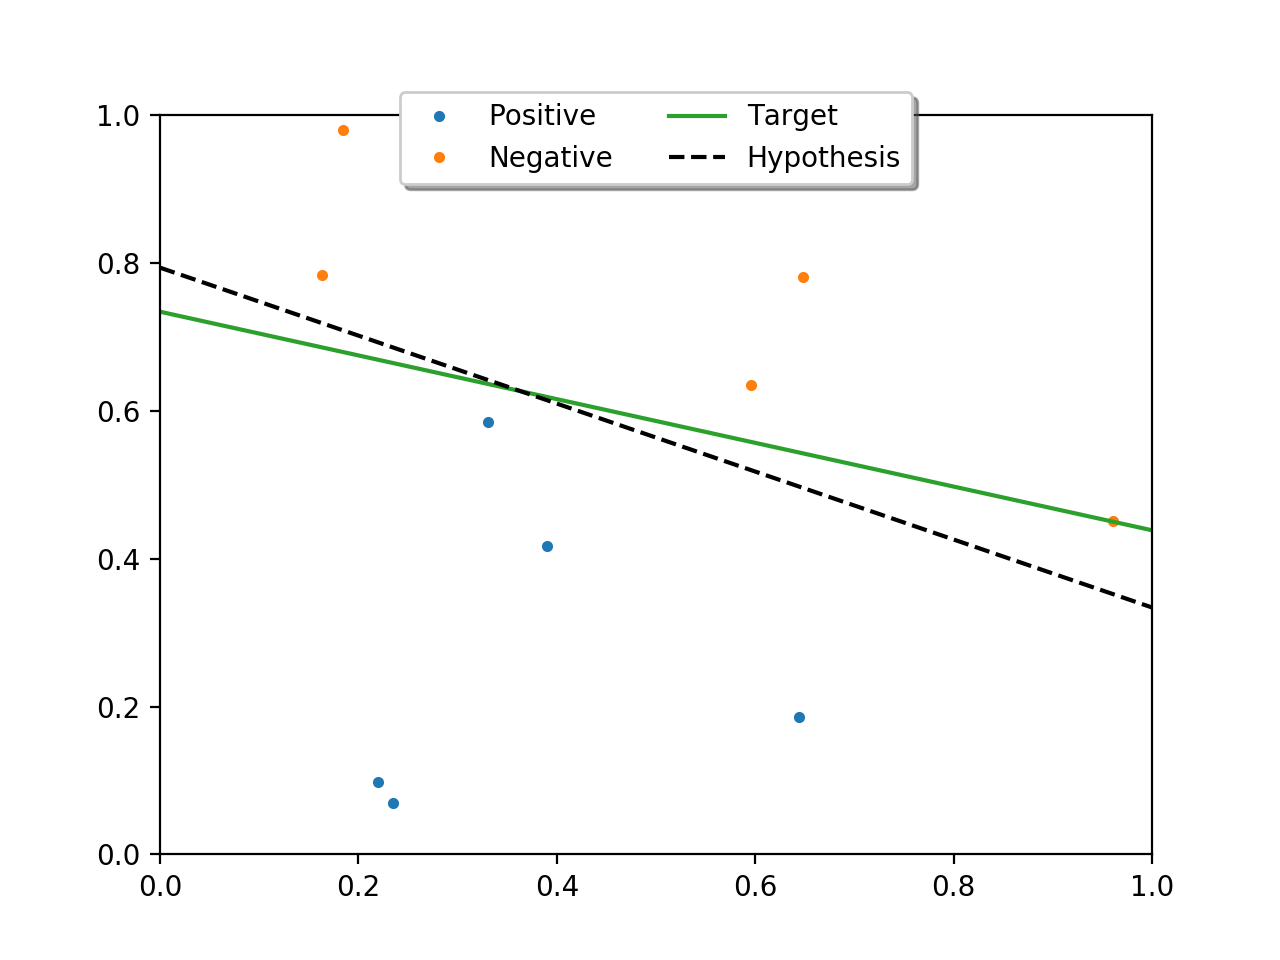
\includegraphics[width=0.65\textwidth]{pla10.png}
	\end{center}
	
	The perceptron code in \texttt{Homework1.py} took 22 iterations on average to converge, and had an average out-of-sample classification error of 0.110.
	
	Therefore the answer is [\textbf{b}].
}
\end{homeworkProblem}

%----------------------------------------------------------------------------------------
%	PROBLEM 8
%----------------------------------------------------------------------------------------

\begin{homeworkProblem}
Which of the following is closest to $\mathbb{P}[f(\mathbf{x}) \neq g(\mathbf{x})]$ for $N = 10$?

\begin{enumerate}
	\item 0.001
	\item 0.01
	\item 0.1
	\item 0.5
	\item 0.8
\end{enumerate} % Question

\problemAnswer{ % Answer
	The answer is [\textbf{c}]. (See answer above)
}
\end{homeworkProblem}

%----------------------------------------------------------------------------------------
%	PROBLEM 9
%----------------------------------------------------------------------------------------

\begin{homeworkProblem}
Now, try $N = 100$. How many iterations does it take on average for the PLA to converge for $N = 100$ training points? Pick the value closest to your results.

\begin{enumerate}
	\item 50
	\item 100
	\item 500
	\item 1000
	\item 5000
\end{enumerate} % Question

\problemAnswer{ % Answer
	Below is a plot showing the target function, training data, and the PLA hypothesis for 100 points.
	
	\begin{center}
		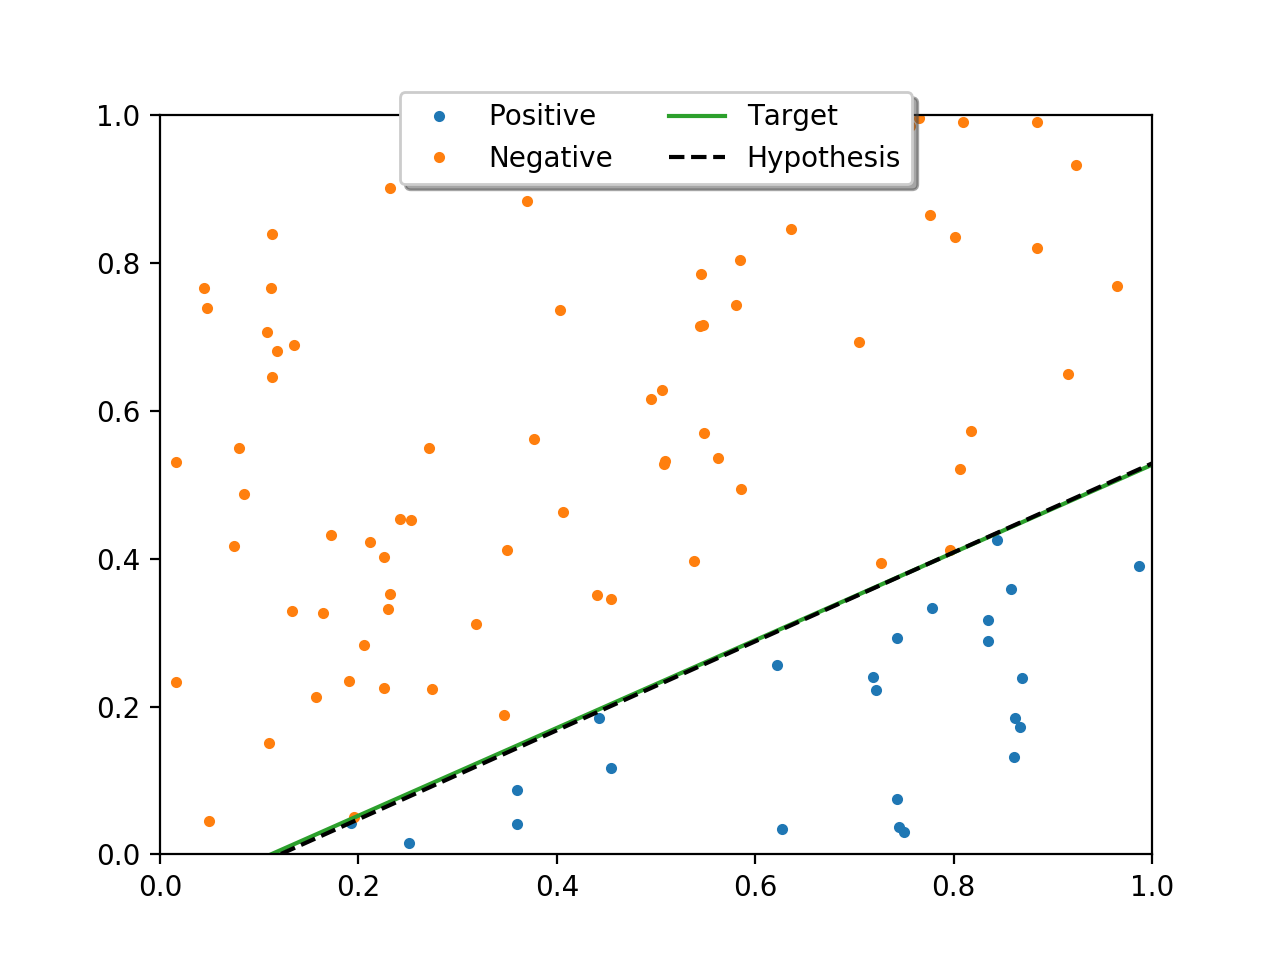
\includegraphics[width=0.65\textwidth]{pla100.png}
	\end{center}
	
	The perceptron code in \texttt{Homework1.py} took 179 iterations on average to converge, and had an average out-of-sample classification error of 0.013.
	
	Therefore the answer is [\textbf{b}].
}
\end{homeworkProblem}

%----------------------------------------------------------------------------------------
%	PROBLEM 10
%----------------------------------------------------------------------------------------

\begin{homeworkProblem}
Which of the following is closest to $\mathbb{P}[f(\mathbf{x}) \neq g(\mathbf{x})]$ for $N = 100$?

\begin{enumerate}
	\item 0.001
	\item 0.01
	\item 0.1
	\item 0.5
	\item 0.8
\end{enumerate} % Question

\problemAnswer{ % Answer
	The answer is [\textbf{b}]. (See answer above)
}
\end{homeworkProblem}

%----------------------------------------------------------------------------------------

\end{document}
